
\subsection{PB}
\subsubsection{Primo Incremento}

\paragraph{Consuntivo Orario}
\begin{center}
	\renewcommand{\arraystretch}{1.8} %aumento ampiezza righe
	\begin{tabular}{ |m{8em}|c|c|c|c|c|c|c| }
	\hline
	\textbf{Membro} & \textbf{Re} & \textbf{Am} &  \textbf{An} &  \textbf{Pt} &  \textbf{Pg} &  \textbf{Ve} &  \textbf{Totale}\\
    \hline
    Irene Benetazzo   & - & 1 (+1)  & 3 (+3)  & 5 (-3)  & 5       & 4 (+1)  & \textbf{18} (+2) \\
    \hline
    Tommaso Berlaffa  & 3 & -       & 1 (+1)  & -       & 8 (-2)  & 1 (+1)  & \textbf{13} \\
    \hline
    Mattia Episcopo   & - & 3 (-1)  & 2 (+2)  & 7       & 4       & 2       & \textbf{18} (+1) \\
    \hline
    Pietro Macrì      & - & - (-4)  & -       & 6 (+1)  & 6 (-1)  & 2       & \textbf{14} (-4)\\
    \hline
    Qi Fan Andrea Pan & - & -       & -       & 8 (+1)  & 6 (-1)  & 2  (-1) & \textbf{16} (-1) \\
    \hline
    Matteo Pillon     & - & -       & -       & 6 (+1)  & 6 (-2)  & 2  (-1) & \textbf{14} (-2) \\
    \hline
    Samuele Rizzato   & - & 2 (+2)  & 2 (+2)  & 6 (-2)  & 5       & 2  (-1) & \textbf{17} (+1) \\
    \hline
    \textbf{Totale ore} & \textbf{3} & \textbf{8} & \textbf{8} (+8) &  \textbf{38} (-2) &  \textbf{40} (-6) &  \textbf{15} (-1) &  \textbf{110} (-3)\\
    \hline
	\end{tabular}
\end{center}
\begin{figure}[H]
    \centering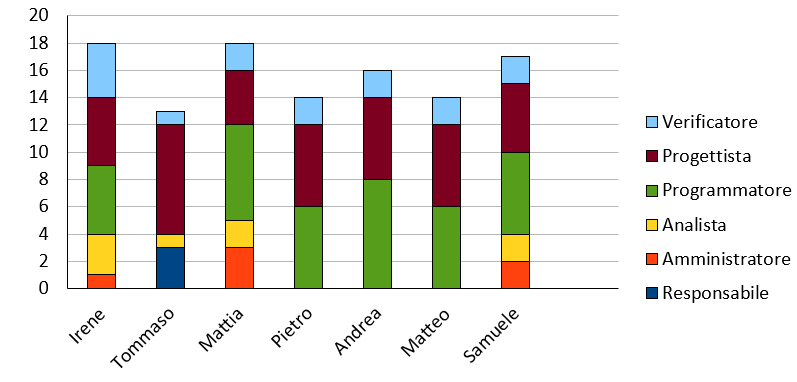
\includegraphics[width=\textwidth, height=\textheight,keepaspectratio]{images/consuntivo/PB-ore.png}
    \caption{PB - Product Baseline - Primo Incremento - consuntivo ripartizione oraria}
\end{figure}

\paragraph{Consuntivo Economico}
\begin{center}
	\renewcommand{\arraystretch}{1.8}
	\begin{tabular}{ |m{6em}|c|c|c|c|c|c|c| }
	\hline
	\textbf{Ruolo} & \textbf{Re} & \textbf{Am} &  \textbf{An} &  \textbf{Pt} &  \textbf{Pg} &  \textbf{Ve} &  \textbf{Totale}\\
    \hline
    Totale ore & 3 & 8 & 8 & 38 & 40 & 14 & \textbf{110}\\
    \hline
    Costo \euro/h & 30\euro/h & 20\euro/h & 25\euro/h & 25\euro/h & 15\euro/h & 15\euro/h & \\
    \hline
    \textbf{Totale costo} & \textbf{90\euro} & \textbf{120\euro} &  \textbf{200\euro} & \textbf{950\euro} &  \textbf{600\euro} &  \textbf{225\euro} &  \textbf{2185\euro} \\
    &  & (-40\euro) & (+200\euro) & (-50\euro) & (-90\euro) & (-25\euro) & (+5\euro) \\
    \hline
	\end{tabular}

    \begin{figure}[H]
        \centering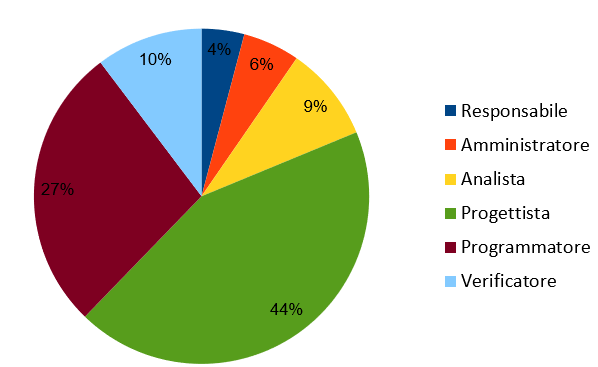
\includegraphics[width=0.7\textwidth, height=0.7\textheight, keepaspectratio]{images/consuntivo/PB-costo.png}
        \caption{PB - Product Baseline - Primo Incremento - consuntivo ripartizione economica}
    \end{figure}
\end{center}

\paragraph{Considerazioni} \hfill \break
L'inizio della fase è stato posticipato, causa revisione con i docenti. A seguito di quest'ultima, 
sono state necessarie ulteriori ore di analista per gestire la correzione e l'analisi di possibili soluzioni della documentazione presentata durante colloquio.\\
L'intera fase di Product Baseline viene quindi temporalmente traslata di conseguenza.

\begin{center}
	\renewcommand{\arraystretch}{1.8}
	\begin{tabular}{ | l |c|c| }
    \hline
    & \textbf{Ore} & \textbf{Costo} \\
	\hline
    \textbf{Consuntivo} & 110 & 2185\euro \\
    \hline
    \textbf{Preventivo} & 113 & 2180\euro \\
    \hline
    \textbf{Bilancio fase} & -3 & -5\euro \\
    \hline
    \textbf{Bilancio complessivo} & \textbf{-39} & \textbf{-890\euro} \\
    \hline
    \end{tabular}
\end{center}
In conclusione il primo incremento della fase Product Baseline termina il 2022-07-20 con un risparmio, relativo
alla fase, di 5€.

\newpage

\subsubsection{Secondo Incremento}

\paragraph{Consuntivo Orario}
\begin{center}
	\renewcommand{\arraystretch}{1.8} %aumento ampiezza righe
	\begin{tabular}{ |m{8em}|c|c|c|c|c|c|c| }
	\hline
	\textbf{Membro} & \textbf{Re} & \textbf{Am} &  \textbf{An} &  \textbf{Pt} &  \textbf{Pg} &  \textbf{Ve} &  \textbf{Totale}\\
    \hline
    Irene Benetazzo   & - & -  & -  & 7  & 5 & 2 (-1) & \textbf{14} \\
    \hline
    Tommaso Berlaffa  & - & - & -  & 6 & 6  & 2 (-1) & \textbf{14} \\
    \hline
    Mattia Episcopo   & 3 & -  & -  & - & 10 & 0 & \textbf{13} \\
    \hline
    Pietro Macrì      & - & -  & - & 5 & 6 & 2 (-1) & \textbf{13} \\
    \hline
    Qi Fan Andrea Pan & - & 2 (-2) & - & 4 & 8 & 2 (-1) & \textbf{16} \\
    \hline
    Matteo Pillon     & - & - & - & 6 & 7 & 2 (-1) & \textbf{15} \\
    \hline
    Samuele Rizzato   & - & 3 (-2) & - & 6 & 5 & 2 (-1) & \textbf{16} \\
    \hline
    \textbf{Totale ore} & \textbf{3} & \textbf{5} (-4) & \textbf{0} &  \textbf{34} &  \textbf{47} &  \textbf{12} (-5) &  \textbf{101} (-9)\\
    \hline
	\end{tabular}
\end{center}
\begin{figure}[H]
    \centering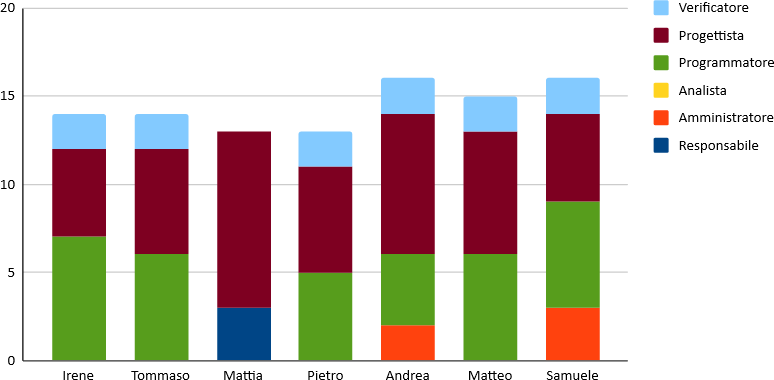
\includegraphics[width=\textwidth, height=\textheight,keepaspectratio]{images/consuntivo/consuntivo-PB-ore-secondo-incremento.png}
    \caption{PB - Product Baseline - Secondo Incremento - consuntivo ripartizione oraria}
\end{figure}

\paragraph{Consuntivo Economico}
\begin{center}
	\renewcommand{\arraystretch}{1.8}
	\begin{tabular}{ |m{6em}|c|c|c|c|c|c|c| }
	\hline
	\textbf{Ruolo} & \textbf{Re} & \textbf{Am} &  \textbf{An} &  \textbf{Pt} &  \textbf{Pg} &  \textbf{Ve} &  \textbf{Totale}\\
    \hline
    Totale ore & 3 & 5 & 0 & 34 & 47 & 12 & \textbf{101}\\
    \hline
    Costo \euro/h & 30\euro/h & 20\euro/h & 25\euro/h & 25\euro/h & 15\euro/h & 15\euro/h & \\
    \hline
    \textbf{Totale costo} & \textbf{90\euro} & \textbf{100\euro} &  \textbf{0\euro} & \textbf{850\euro} &  \textbf{705\euro} &  \textbf{180\euro} &  \textbf{1925\euro} \\
    &  & (-80\euro) & & & & (-75\euro) & (-155\euro) \\
    \hline
	\end{tabular}

    \begin{figure}[H]
        \centering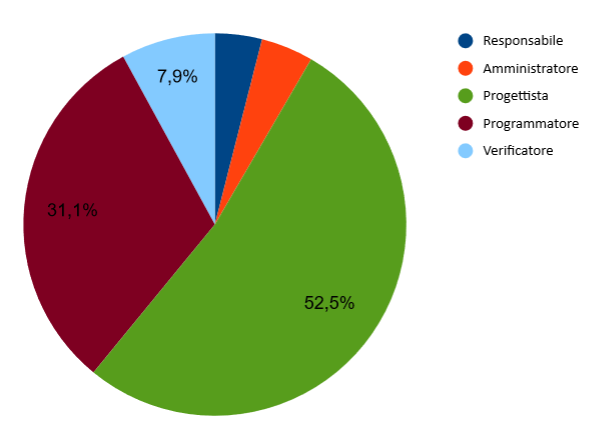
\includegraphics[width=0.7\textwidth, height=0.7\textheight, keepaspectratio]{images/consuntivo/consuntivo-PB-costo-secondo-incremento.png}
        \caption{PB - Product Baseline - Secondo Incremento - consuntivo ripartizione economica}
    \end{figure}
\end{center}

\paragraph{Considerazioni} \hfill \break
Il secondo incremento era stato sovrastimato in sede di preventivo, sia come ore che come costi. In termini di ore c'è stato un discreto risparmio di tempo per i ruoli di verificatore (4) e amministratore (5) che hanno portato ad un risparmio complessivo di 9 ore.
\begin{center}
	\renewcommand{\arraystretch}{1.8}
	\begin{tabular}{ | l |c|c| }
    \hline
    & \textbf{Ore} & \textbf{Costo} \\
	\hline
    \textbf{Consuntivo} & 101 & 1925\euro \\
    \hline
    \textbf{Preventivo} & 110 & 2080\euro \\
    \hline
    \textbf{Bilancio fase} & -9 & -155\euro \\
    \hline
    \textbf{Bilancio complessivo} & \textbf{-48} & \textbf{-1045\euro} \\
    \hline
    \end{tabular}
\end{center}
In conclusione il secondo incremento della fase Product Baseline termina il 2022-08-03 con un risparmio economico, relativo alla fase, di 155€.

\subsubsection{Terzo Incremento}

\paragraph{Consuntivo Orario}
\begin{center}
	\renewcommand{\arraystretch}{1.8} %aumento ampiezza righe
	\begin{tabular}{ |m{8em}|c|c|c|c|c|c|c| }
	\hline
	\textbf{Membro} & \textbf{Re} & \textbf{Am} &  \textbf{An} &  \textbf{Pt} &  \textbf{Pg} &  \textbf{Ve} &  \textbf{Totale}\\
    \hline
    Irene Benetazzo   & - & - & - & 4 & 5 & 3 & \textbf{12} \\
    \hline
    Tommaso Berlaffa  & - & - & - & 5 & 4 & 3 & \textbf{12} \\
    \hline
    Mattia Episcopo   & - & 5 & - & 3 & 5 & 2 & \textbf{15} \\
    \hline
    Pietro Macrì      & 3 & - & - & - & 7 & - & \textbf{10} \\
    \hline
    Qi Fan Andrea Pan & - & - & - & 4 & 5 & 3 & \textbf{12} \\
    \hline
    Matteo Pillon     & - & 4 & - & 5 & 3 & 2 & \textbf{14} \\
    \hline
    Samuele Rizzato   & - & - & - & 5 & 5 & 3 & \textbf{13} \\
    \hline
    \textbf{Totale ore} & \textbf{3} & \textbf{9} & \textbf{0} & \textbf{26} & \textbf{34} & \textbf{16} & \textbf{88} \\
    \hline
	\end{tabular}
\end{center}
\begin{figure}[H]
    \centering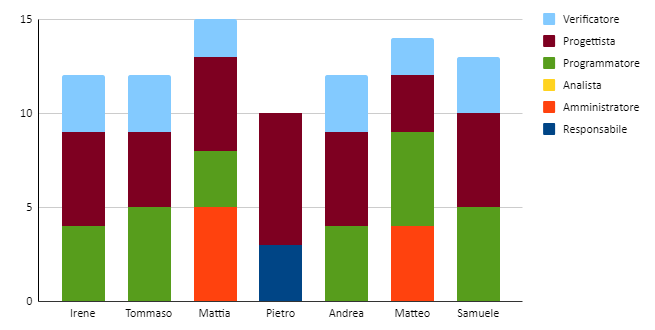
\includegraphics[width=\textwidth, height=\textheight,keepaspectratio]{images/consuntivo/consuntivo-PB-ore-terzo-incremento.png}
    \caption{PB - Product Baseline - Terzo Incremento - consuntivo ripartizione oraria}
\end{figure}

\paragraph{Consuntivo Economico}
\begin{center}
	\renewcommand{\arraystretch}{1.8}
	\begin{tabular}{ |m{6em}|c|c|c|c|c|c|c| }
	\hline
	\textbf{Ruolo} & \textbf{Re} & \textbf{Am} &  \textbf{An} &  \textbf{Pt} &  \textbf{Pg} &  \textbf{Ve} &  \textbf{Totale}\\
    \hline
    Totale ore & 3 & 9 & 0 & 26 & 34 & 16 & \textbf{88}\\
    \hline
    Costo \euro/h & 30\euro/h & 20\euro/h & 25\euro/h & 25\euro/h & 15\euro/h & 15\euro/h & \\
    \hline
    \textbf{Totale costo} & \textbf{90\euro} & \textbf{180\euro} &  \textbf{0\euro} & \textbf{650\euro} &  \textbf{510\euro} &  \textbf{240\euro} &  \textbf{1670\euro} \\
    \hline
	\end{tabular}

    \begin{figure}[H]
        \centering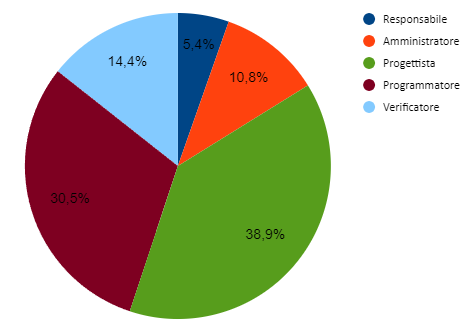
\includegraphics[width=0.7\textwidth, height=0.7\textheight, keepaspectratio]{images/consuntivo/consuntivo-PB-costo-terzo-incremento.png}
        \caption{PB - Product Baseline - Terzo Incremento - consuntivo ripartizione economica}
    \end{figure}
\end{center}

\paragraph{Considerazioni} \hfill \break
Il terzo incremento era stato correttamente stimato in sede di preventivo, sia in termini di numero di ore sia 
in termini di distribuzione delle ore. Il consuntivo di questo incremento si conclude dunque in pari.
\begin{center}
	\renewcommand{\arraystretch}{1.8}
	\begin{tabular}{ | l |c|c| }
    \hline
    & \textbf{Ore} & \textbf{Costo} \\
	\hline
    \textbf{Consuntivo} & 88 & 1670\euro \\
    \hline
    \textbf{Preventivo} & 88 & 1670\euro \\
    \hline
    \textbf{Bilancio fase} & 0 & 0\euro \\
    \hline
    \textbf{Bilancio complessivo} & \textbf{0} & \textbf{0\euro} \\
    \hline
    \end{tabular}
\end{center}
In conclusione il terzo incremento della fase Product Baseline termina il 2022-08-17 in pari.
\newpage

\subsubsection{Quarto Incremento}

\paragraph{Consuntivo Orario}
\begin{center}
	\renewcommand{\arraystretch}{1.8} %aumento ampiezza righe
	\begin{tabular}{ |m{8em}|c|c|c|c|c|c|c| }
	\hline
	\textbf{Membro} & \textbf{Re} & \textbf{Am} &  \textbf{An} &  \textbf{Pt} &  \textbf{Pg} &  \textbf{Ve} &  \textbf{Totale}\\
    \hline
    Irene Benetazzo   & 1 & 3  & - & 5 & 4 & 3 & \textbf{16} \\
    \hline
    Tommaso Berlaffa  & 1 & 4  & - & 4 & 5 & 3 & \textbf{17} \\
    \hline
    Mattia Episcopo   & 1 & - & - & 4 & 4 & 3 & \textbf{12} \\
    \hline
    Pietro Macrì      & 1 & 3  & - & 6 & 6 & 3 & \textbf{19} \\
    \hline
    Qi Fan Andrea Pan & 1 & - & - & 6 & 6 & 3 & \textbf{16} \\
    \hline
    Matteo Pillon     & 4 &3  & - & - & 6 & - & \textbf{13} \\
    \hline
    Samuele Rizzato   & 1 &2  &2 & 4 & 4 & 3 & \textbf{16} \\
    \hline
    \textbf{Totale ore} & \textbf{10} & \textbf{15} & \textbf{2} & \textbf{29} & \textbf{35} & \textbf{18} & \textbf{109} \\
    \hline
	\end{tabular}
\end{center}
\begin{figure}[H]
    \centering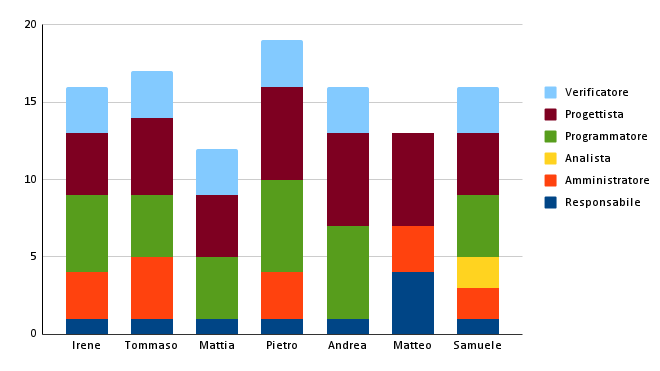
\includegraphics[width=\textwidth, height=\textheight,keepaspectratio]{images/consuntivo/consuntivo-PB-ore-quarto-incremento.png}
    \caption{PB - Product Baseline - Quarto Incremento - consuntivo ripartizione oraria}
\end{figure}
\newpage

\paragraph{Consuntivo Economico}
\begin{center}
	\renewcommand{\arraystretch}{1.8}
	\begin{tabular}{ |m{6em}|c|c|c|c|c|c|c| }
	\hline
	\textbf{Ruolo} & \textbf{Re} & \textbf{Am} &  \textbf{An} &  \textbf{Pt} &  \textbf{Pg} &  \textbf{Ve} &  \textbf{Totale}\\
    \hline
    Totale ore & 10 & 15 & 2 & 29 & 35 & 18 & \textbf{109}\\
    \hline
    Costo \euro/h & 30\euro/h & 20\euro/h & 25\euro/h & 25\euro/h & 15\euro/h & 15\euro/h & \\
    \hline
    \textbf{Totale costo} & \textbf{300\euro} & \textbf{300\euro} &  \textbf{50\euro} & \textbf{725\euro} &  \textbf{525\euro} &  \textbf{270\euro} &  \textbf{2170\euro} \\
    \hline
	\end{tabular}

    \begin{figure}[H]
        \centering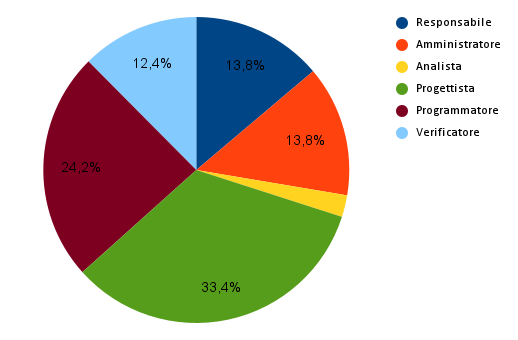
\includegraphics[width=0.7\textwidth, height=0.7\textheight, keepaspectratio]{images/consuntivo/consuntivo-PB-costo-quarto-incremento.png}
        \caption{PB - Product Baseline - Quarto Incremento - consuntivo ripartizione economica}
    \end{figure}
\end{center}

\paragraph{Considerazioni} \hfill \break
Il quarto incremento non è stato correttamente stimato in sede di preventivo, sia in termini di numero di ore sia 
in termini di distribuzione delle ore. Il consuntivo di questo incremento si conclude dunque con l'utilizzo di 12 ore in più rispetto al preventivo, aventi un costo totale per questa fase di 270\euro.
\begin{center}
	\renewcommand{\arraystretch}{1.8}
	\begin{tabular}{ | l |c|c| }
    \hline
    & \textbf{Ore} & \textbf{Costo} \\
	\hline
    \textbf{Consuntivo} & 109 & 2170\euro \\
    \hline
    \textbf{Preventivo} & 97 & 1900\euro \\
    \hline
    \textbf{Bilancio fase} & +12 & +270\euro \\
    \hline
    \textbf{Bilancio complessivo} & \textbf{12} & \textbf{+270\euro} \\
    \hline
    \end{tabular}
\end{center}
In conclusione il quarto incremento della fase Product Baseline termina il 2022-08-30 con un costo economico, relativo alla fase, di 270\euro.

\subsubsection{Complessivo PB}

\paragraph{Consuntivo Orario}
\begin{center}
	\renewcommand{\arraystretch}{1.8} %aumento ampiezza righe
	\begin{tabular}{ |m{8em}|c|c|c|c|c|c|c| }
	\hline
	\textbf{Membro} & \textbf{Re} & \textbf{Am} &  \textbf{An} &  \textbf{Pt} &  \textbf{Pg} &  \textbf{Ve} &  \textbf{Totale}\\
    \hline
    Irene Benetazzo   & 1 & 4  & 3 & 21 & 19 & 12 & \textbf{60} \\
    \hline
    Tommaso Berlaffa  & 4 & 4  & 1 & 15 & 23 & 9 & \textbf{56} \\
    \hline
    Mattia Episcopo   & 4 & 8 & 2 & 14 & 23 & 7 & \textbf{58} \\
    \hline
    Pietro Macrì      & 4 & 3  & - & 17 & 25 & 7 & \textbf{56} \\
    \hline
    Qi Fan Andrea Pan & 1 & 2 & - & 22 & 25 & 10 & \textbf{60} \\
    \hline
    Matteo Pillon     & 4 &7  & - & 17 & 22 & 6 & \textbf{56} \\
    \hline
    Samuele Rizzato   & 1 &7  &4 & 21 & 19 & 10 & \textbf{62} \\
    \hline
    \textbf{Totale ore} & \textbf{19} & \textbf{35} & \textbf{10} & \textbf{127} & \textbf{156} & \textbf{61} & \textbf{408} \\
    \hline
	\end{tabular}
\end{center}
\begin{figure}[H]
    \centering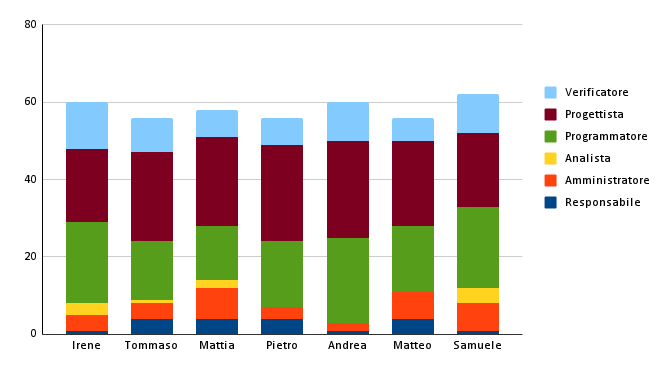
\includegraphics[width=\textwidth, height=\textheight,keepaspectratio]{images/consuntivo/consuntivo-PB-ore-totale.png}
    \caption{PB - Product Baseline - Complessivo PB - consuntivo ripartizione oraria}
\end{figure}
\newpage

\paragraph{Consuntivo Economico}
\begin{center}
	\renewcommand{\arraystretch}{1.8}
	\begin{tabular}{ |m{6em}|c|c|c|c|c|c|c| }
	\hline
	\textbf{Ruolo} & \textbf{Re} & \textbf{Am} &  \textbf{An} &  \textbf{Pt} &  \textbf{Pg} &  \textbf{Ve} &  \textbf{Totale}\\
    \hline
    Totale ore & 19 & 35 & 10 & 127 & 156 & 61 & \textbf{408}\\
    \hline
    Costo \euro/h & 30\euro/h & 20\euro/h & 25\euro/h & 25\euro/h & 15\euro/h & 15\euro/h & \\
    \hline
    \textbf{Totale costo} & \textbf{570\euro} & \textbf{700\euro} &  \textbf{250\euro} & \textbf{3175\euro} &  \textbf{2340\euro} &  \textbf{915\euro} &  \textbf{7950\euro} \\
    \hline
	\end{tabular}

    \begin{figure}[H]
        \centering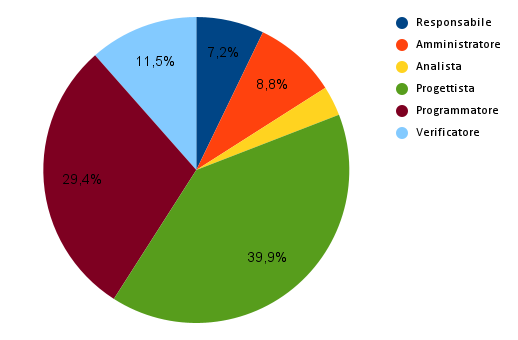
\includegraphics[width=0.7\textwidth, height=0.7\textheight, keepaspectratio]{images/consuntivo/consuntivo-PB-costo-totale.png}
        \caption{PB - Product Baseline - Complessivo PB - consuntivo ripartizione economica}
    \end{figure}
\end{center}

\paragraph{Considerazioni} \hfill \break
La Product Baseline termina con un ritardo di 35 giorni rispetto alla pianificazione, 15 dei quali dovuti alla precedente revisione RTB che ha richiesto una fase aggiuntiva non prevista e 20 dovuti a ritardi nell'avanzamento del lavoro, con un esborso economico di 120€ in più del previsto. Il numero totale di ore lavorate è stato esattamente quanto previsto, questo perchè la distribuzione interna della ore tra i ruoli non è stata preventivata correttamente.

\begin{center}
	\renewcommand{\arraystretch}{1.8}
	\begin{tabular}{ | l |c|c| }
    \hline
    & \textbf{Ore} & \textbf{Costo} \\
	\hline
    \textbf{Consuntivo} & 408 & 7950\euro \\
    \hline
    \textbf{Preventivo} & 408 & 7830\euro \\
    \hline
    \textbf{Bilancio fase} & 0 & +120\euro \\
    \hline
    \textbf{Bilancio complessivo} & \textbf{0} & \textbf{0\euro} \\
    \hline
    \end{tabular}
\end{center}
In conclusione la Product Baseline termina il 2022-08-30.

\newpage
\paragraph{Preventivo a Finire} \hfill \break

\begin{center}
	\renewcommand{\arraystretch}{1.8}
	\begin{tabular}{ | l |c|c|c| }
    \hline
    \textbf{Ruolo} & \textbf{Preventivo attuale} & \textbf{Preventivo iniziale}  & \textbf{Differenza economica}\\
	\hline
    \textbf{Responsabile} & 40 & 40 & 0\euro \\
    \hline
    \textbf{Amministratore} & 90 & 100 & -200\euro \\
    \hline
    \textbf{Analista} & 70 & 100 & -750\euro \\
    \hline
    \textbf{Progettista} & 170 & 160 & 250\euro \\
    \hline
    \textbf{Programmatore} & 190 & 160 & 450\euro \\
    \hline
    \textbf{Verificatore} & 140 & 140 & 0\euro \\
    \hline
    \textbf{Totale} & \textbf{700} & \textbf{700} & \textbf{-250\euro} \\
    \hline
    \end{tabular}
\end{center}
Non è cambiato il numero complessivo di ore ma la distribuzione interna e data la differenza di prezzo tra i vari ruoli, ciò porta ad un risparmio di 250 \euro rispetto al preventivo iniziale. \newline
Il preventivo della macrofase Product Baseline (\$5.2) è stato stilato basandosi sul preventivo attuale.